\documentclass[11 pt,xcolor=dvipsnames,xcolor=table]{beamer}
\usetheme[
	bullet=square,		% Other option: square
	bigpagenumber,		% circled page number on lower right
	topline=true,			% colored bar at the top of the frame 
	shadow= true,			% Shading for beamer blocks
	watermark=BG_lower,	% png file for the watermark
	]{Flip}

\setbeameroption{hide notes}

\newcommand{\titleimage}{title}			% Custom title 
\newcommand{\tanedo}{tanedolight}		% Custom author name
\newcommand{\CMSSMDM}{CMSSMDMlight.png}	% light background plot
\usepackage{picins}

%%%%%%%%%%
% FONTS %
%%%%%%%%%%

\usepackage{sfmath}		

%%%%%%%%%%%%%%%%%%%%%%%%
% Usual LaTeX Packages %
%%%%%%%%%%%%%%%%%%%%%%%%

\usepackage{amsmath}
\usepackage{amsfonts}
\usepackage{amssymb}
\usepackage{graphicx}
\usepackage{mathrsfs} 			% For Weinberg-esque letters
\usepackage{cancel}				% For "SUSY-breaking" symbol
\usepackage{slashed}            % for slashed characters in math mode
\usepackage{amsthm}				% For theorem environment
\usepackage{multirow}			% For multi row cells in table
%\usepackage{tikzfeynman}		% For Feynman diagrams
\usepackage{graphics}
\usepackage{listings}
\usepackage{mathpazo}
\usepackage{media9}
\addmediapath{./movies/}
\graphicspath{{images/}}	% Put all images in this directory. Avoids clutter.
\setbeamercovered{transparent}


\usetikzlibrary{backgrounds}
\usetikzlibrary{mindmap,trees}	% For mind map
% http://www.texample.net/tikz/examples/computer-science-mindmap/


% SOME COMMANDS THAT I FIND HANDY

\newcommand{\comment}[1]{\textcolor{comment}{\footnotesize{#1}\normalsize}} % comment mild
\newcommand{\Comment}[1]{\textcolor{Comment}{\footnotesize{#1}\normalsize}} % comment bold
\newcommand{\COMMENT}[1]{\textcolor{COMMENT}{\footnotesize{#1}\normalsize}} % comment crazy bold
\newcommand{\Alert}[1]{\textcolor{Alert}{#1}} % louder alert
\newcommand{\ALERT}[1]{\textcolor{ALERT}{#1}} % loudest alert
%% "\alert" is already a beamer pre-defined
%\newcommand{\blue}[1]{\textcolor{profound}{#1}}



\defbeamertemplate*{title page}{customized}[1][]
{\begin{center}
  {\fontfamily{phv}\selectfont \Large{{\textcolor{brunfonce}{\inserttitle}}}}\par
  \usebeamerfont{subtitle}\usebeamercolor[fg]{subtitle}\insertsubtitle\par
  \bigskip
  \usebeamerfont{author}\alert{\insertauthor}\par
  \usebeamerfont{institute}\insertinstitute\par
  \usebeamerfont{date}\insertdate\par
  \usebeamercolor[fg]{titlegraphic}\inserttitlegraphic
  \end{center}
}
\title[ECCM-ECFD 2018]{{\normalsize Parallel Multigrid Solver for Finite Elements using B-Spline}}

\author[Jalal Lakhlili]{\underline{Jalal Lakhlili}\footnotemark[1],  Yaman G\"u\c{c}l\"u\footnotemark[1], Ahmed Ratnani\footnotemark[1] \\ (Tran-Minh Tran\footnotemark[2])}

\institute{ 
  \footnotetext[1]{Max-Planck-Institut f\"ur Plasmaphysik Garching, Germany.} 
  \footnotetext[2]{Suiss Plasma Center - \'Ecole Polytechnique F\'ed\'erale de Lausanne, Switzerland.} 
  }

\date{{\color{white} -} \\ ECCM-ECFD 2018 \\ M.S. Mathematical aspects of isogeometric analysis
 \\ Glasgow - \today}


%%%%%%%%%%%%%%%
%  ARA
%\setbeamertemplate{itemize/enumerate body begin}{\normalsize}
%\setbeamertemplate{itemize/enumerate subbody begin}{\tiny}

\usepackage{pifont}
\usepackage{color}
\usepackage[table]{xcolor}
\usepackage{xcolor}
\definecolor{darkgreen}{RGB}{0,142,128}
\definecolor{bleufonce}{RGB}{20,20,144}
\definecolor{vertCEA_light}{RGB}{249,253,246}
\definecolor{vertCEA_Light}{RGB}{230,246,216}
%\definecolor{vertCEA_light}{RGB}{199,235,169}
\definecolor{flameOrange}{RGB}{255,243,224}
\definecolor{orangeCEA_Light}{RGB}{255,220,167}

% tmp
\definecolor{bleufonce}{RGB}{20,20,144}
\definecolor{vertCEA_light}{RGB}{249,253,246}
\definecolor{vertCEA_Light}{RGB}{230,246,216}
%\definecolor{vertCEA_light}{RGB}{199,235,169}
\definecolor{orangeCEA_light}{RGB}{255,243,224}
\definecolor{orangeCEA_Light}{RGB}{255,220,167}
\definecolor{darkgreen}{RGB}{0,142,128}
\definecolor{bleufonce}{RGB}{0,142,128}
\definecolor{orangelight}{RGB}{0,142,128}
%


\usepackage[framemethod=tikz]{mdframed}
\usetikzlibrary{decorations.pathmorphing,calc}
\usepackage{lipsum}% just to generate text for the example

\newcommand{\dr}{\partial_R}
\newcommand{\dz}{\partial_z}
\newcommand{\dphi}{\partial_{\varphi}}
\newcommand{\ephi}{e_{\varphi}}
\newcommand{\lp}{\triangle_{pol}}
\newcommand{\lpp}{\triangle_{pol}^2}
\newcommand{\lpm}{\triangle_{pol}^{-1}}
\newcommand{\gs}{\triangle^{*}}
\newcommand{\U}{\mathbf{U}}
\newcommand{\V}{\mathbf{V}}
\newcommand{\vB}{\mathbf{B}}
\newcommand{\vJ}{\mathbf{J}}
\newcommand{\vE}{\mathbf{E}}
\newcommand{\rot}{\nabla \times}
\newcommand{\er}{e_R}
\newcommand{\ez}{e_z}
\newcommand{\rhoh}{R^2 \rho}
\newcommand{\curls}{\mathrm{curl}\,}
\newcommand{\divs}{\mathrm{div}\,}
\newcommand{\divv}{\mathbf{div}\,}
\newcommand{\curlv}{\mathbf{curl}\,}
\newcommand{\xx}{\mathbf{x}\,}
\newcommand{\vv}{\mathbf{v}\,}
\newcommand{\ff}{\mathbf{f}}
\newcommand{\uu}{\mathbf{u}}
\newcommand{\nn}{\mathbf{n}}
\newcommand{\EE}{\mathbf{E}}
\newcommand{\FF}{\mathbf{F}}
\newcommand{\JJ}{\mathbf{J}}
\newcommand{\HH}{\mathbf{H}}
\newcommand{\BB}{\mathbf{B}}
\newcommand{\DD}{\mathbf{D}}
\newcommand{\xixi}{\boldsymbol{\xi}\,}
\newcommand{\Alt}{\mathrm{Alt}\,}
\newcommand{\diff}{\mathrm{d}\,}
\newcommand{\trace}{\mathrm{Tr}\,}
\newcommand{\volume}{\mathrm{vol}\,}
\newcommand{\id}{\mathrm{id}\,}
\newcommand{\hess}{\mathbf{Hess}}
\newcommand{\Hdiv}{H(\mbox{div}, \Omega)}
\newcommand{\Hcurl}{H(\mbox{curl}, \Omega)}
\newcommand{\Hcurlzero}{H_0(\mbox{curl}, \Omega)}
\newcommand{\Hdivzero}{H_0(\mbox{div}, \Omega)}
\newcommand{\fracp}[2]{\frac{\partial #1}{\partial #2}}  
\newcommand{\dd}{\,\mathrm{d}}
\newcommand{\Rotv}{\boldsymbol{\nabla} \times}
\newcommand{\Rots}{\nabla \times}
\newcommand{\Div}{\nabla \cdot}
\newcommand{\Grad}{\boldsymbol{\nabla}}
\newcommand{\dt}{\partial_t}
\newcommand{\ds}{\displaystyle}
\newcommand{\diffcolor}{\textcolor{blue}}
\newcommand{\twofluidcolor}{\textcolor{magenta}}
\newcommand{\termsourcecolor}{\textcolor{darkgreen}}
\newcommand{\st}{\overline{\overline{\mathbf{\Pi}}}}
\newtheorem{proposition}{Proposition}
\newcommand\tab[1][0.25cm]{\hspace*{#1}}

\newcommand{\Vspline}{\mathcal{S}^{p,p,p}}
\newcommand{\Xspline}{\mathcal{S}^{p-1,p-1,p-1}}

\newcommand{\Wcurlspline}{
  \begin{pmatrix}
    \mathcal{S}^{p-1,p,p} \\ 
    \mathcal{S}^{p,p-1,p} \\ 
    \mathcal{S}^{p,p,p-1}
  \end{pmatrix}
}

\newcommand{\Wdivspline}{
  \begin{pmatrix}
    \mathcal{S}^{p,p-1,p-1} \\ 
    \mathcal{S}^{p-1,p,p-1} \\ 
    \mathcal{S}^{p-1,p-1,p}
  \end{pmatrix}
}


%\newcommand{\HcurlBS}{\mathcal{S}_{\alpha,\alpha-1,\alpha-1}^{p,p-1,p-1} \times \mathcal{S}_{\alpha-1,\alpha,\alpha-1}^{p-1,p,p-1} \times \mathcal{S}_{\alpha-1,\alpha-1,\alpha}^{p-1,p-1,p}}
%
%%\newcommand{\HdivBS}{\mathcal{S}_{\alpha,\alpha-1,\alpha-1}^{p,p-1,p-1} \times \mathcal{S}_{\alpha-1,\alpha,\alpha-1}^{p-1,p,p-1} \times \mathcal{S}_{\alpha-1,\alpha-1,\alpha}^{p-1,p-1,p}}
%\newcommand{\HdivBS}{\mathcal{S}_{\alpha-1,\alpha,\alpha}^{p-1,p,p} \times \mathcal{S}_{\alpha,\alpha-1,\alpha}^{p,p-1,p} \times \mathcal{S}_{\alpha,\alpha,\alpha-1}^{p,p,p-1}}
%\newcommand{\HunBS}{\mathcal{S}_{\alpha,\alpha,\alpha}^{p,p,p}}
%\newcommand{\LdeuxBS}{\mathcal{S}_{\alpha-1,\alpha-1,\alpha-1}^{p-1,p-1,p-1}}

% --- backup unnumbered frames
\newcommand{\backupbegin}{
   \newcounter{finalframe}
   \setcounter{finalframe}{\value{framenumber}}
}
\newcommand{\backupend}{
   \setcounter{framenumber}{\value{finalframe}}
}
% ---

\newcommand\wavydecor{%
    \draw[decoration={coil,aspect=0.1,segment length=5pt,amplitude=0.8pt},decorate,line width=1.5pt,black]
      (O|-P) -- (O);
}

\newmdenv[
hidealllines=true,
innerleftmargin=10pt,
innerrightmargin=0pt,
innertopmargin=0pt,
innerbottommargin=0pt,
leftmargin=-10pt,
skipabove=.5\baselineskip,
skipbelow=.5\baselineskip,
singleextra={\wavydecor},
firstextra={\wavydecor},
secondextra={\wavydecor},
middleextra={\wavydecor}
]{wavysbar}
%%%%%%%%%%%%%%%

%\usefonttheme[onlysmall]{structurebold}

\usepackage{subfigure}
\def\JPicScale{0.25}
\begin{document}

%%%%%%%%%%%%%%%%%%%%%%%%
% Additional  settings %
%%%%%%%%%%%%%%%%%%%%%%%%

%% To use external nodes; http://www.texample.net/tikz/examples/beamer-arrows/
\tikzstyle{every picture}+=[remember picture]


%%%%%%%%%%%%%%%%%%%%%%%%
% Actual content below %
%%%%%%%%%%%%%%%%%%%%%%%%

%% It's much nicer to have all the content in a separate file
% DO NOT COMPILE THIS FILE DIRECTLY!
% This is included by the the driver file (FlipBeamerTemplate.tex).

\maketitle

%******************************************************************
%\begin{frame}{Context and motivation}


%\end{frame}
%******************************************************************


%******************************************************************
\begin{frame}
\frametitle{Outline}

\begin{enumerate}[I]
  \item <1-2> Multigrid (MG) using B-Splines 
  \item <1> 2D parallelization of the MG solver
\end{enumerate}
%
\end{frame}
%******************************************************************


%******************************************************************
\begin{frame}
\frametitle{Overview}
Multigrid methods are efficient solvers/preconditioners for linear or
nonlinear systems of equations derived from discretizations of elliptic PDEs, i.e. find $u \in U$ such that:

\begin{align*}
a(u, v ) = f (v ) \quad  \forall v \in V,
\end{align*}

or equivalently:
\begin{align*}
	Ax = b.
\end{align*}

Theoretically, in optimal case, their numerical complexity is $\mathcal{O}(n)$.\\

\end{frame}
%******************************************************************


%******************************************************************
\begin{frame}
\frametitle{Main idea}
Geometric multigrid is based on a fine-to-coarse grid/FE-space
hierarchy of the problem.
\begin{figure}
 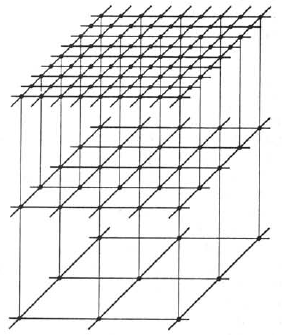
\includegraphics[scale=0.45]{figures/grids}
\end{figure}

\end{frame}
%******************************************************************

%******************************************************************
\begin{frame}
\frametitle{Ingredients}
\begin{itemize}
  \item Mesh hierarchy: fine to coarse.
  \begin{itemize}
  	\item[\ding{224}] We discretise the PDE in the fine mesh.
  \end{itemize}

  \item Restriction operator: mapping from fine to coarse.
  \item Prolongation operator: mapping from coarse to fine.
  \item Smoother on each level.
  \item Coarse grid solver.
\end{itemize}

\end{frame}
%******************************************************************

%******************************************************************
\begin{frame}
\frametitle{Inter-grid operations}

\begin{flushright}
$\triangleright$  {\scriptsize C. de Boor (2001)}
\end{flushright}
  \small
Prolongation and Restriction are based on the knot insertion algorithm.
  \begin{itemize}

\item We consider a nested sequence of knot vectors $T_0 ~ \subset ~ T_1 ~ \subset ~\dots ~ \subset ~T_n$. 
\item We compute the knot insertion matrix $P_i^{i+1}$ from $T_i$ to $T_{i+1}$.
\item We obtain the insertion matrix from $T_0$ to $T_{n}$ by:
\begin{align*}
\mathcal{P} := P_0^{n} = P_0^{1} ~P_1^{2} ~ \dots ~ P_{n-1}^{n},
\end{align*}
which correspands to the \textbf{Prolongation} operator. 

  \begin{itemize}
\item[\ding{224}] In 2D, if $\mathcal{P}_1$, $\mathcal{P}_2$ denote the transfer operators for each direction, then the Prolongation operator is defined as the Kronecker product: 
\begin{align*}
\mathcal{P} := \mathcal{P}_1 \otimes \mathcal{P}_2.
\end{align*}

\item[\ding{224}]  The \textbf{Restriction} operator is then defined as: $\mathcal{R} := \mathcal{P}^T$.
  \end{itemize}
  
\end{itemize}
\end{frame}
%******************************************************************



%******************************************************************
\begin{frame}
\frametitle{V-cycle algorithm}
\begin{enumerate}
  \item {Iterate: \rule{0.8cm}{0pt} ${\texttt x_f :=  pcg^{\nu_1}(A_f, x_0, b_f)}$}
  \item Get residual: \rule{0cm}{0pt} ${\texttt r_f = b_f - A_f x_f}$
  \item Coarsen: \rule{0.6cm}{0pt} ${\texttt r_c = R r_f}$
  \item Solve: \rule{1cm}{0pt} ${\texttt A_c e_c = r_c}$
  \item Correct: \rule{0.7cm}{0pt} ${\texttt x_f := x_f + Pe_c}$
  \item Iterate: \rule{0.8cm}{0pt} ${\texttt x_f := pcg^{\nu_2}(A_f, x_f, b_f)}$
\end{enumerate}

\begin{figure}
 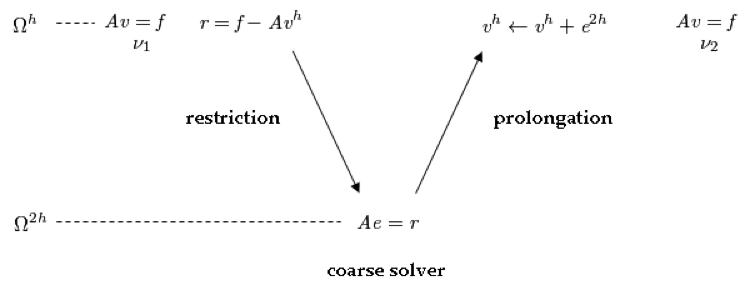
\includegraphics[scale=0.4]{figures/v-cycle1}
\end{figure}

\begin{footnotesize}
*$A_c = RA_fP$ is the coarse-grid version of $A$.
\end{footnotesize}
\end{frame}
%******************************************************************

%******************************************************************
\begin{frame}
\frametitle{Post-smoothing}
\begin{flushright}
$\triangleright$  {\scriptsize Garoni, Manni, Pelosi, Serra-Capizzano and  Speleers (2014)}
\end{flushright}
  \small
The Stiffness matrix for a B-Splines discretization presents a pathology in high frequencies. 
 \begin{itemize}
\item[\ding{224}] Change the post-smoother in the Multigrid algorithm using \textbf{PCG} with the following preconditioner:
\begin{align*}
 T[\mathfrak{m}_{p-1}] \otimes T[\mathfrak{m}_{p-1}].
  \end{align*}
$T[\mathfrak{m}_{p-1}]$ is the Toeplitz matrix associated to the symbol $\mathfrak{m}_{p-1}$ defined as
\begin{align*}
    \mathfrak{m}_p(x, \theta) := \mathfrak{m}_p(\theta) = \phi_{2p+1}(p+1) + 2 \sum_{k=1}^p \phi_{2p+1}(p+1-k) \cos(k \theta),
 \end{align*}

where $\phi_{2p+1}$ is the c\textbf{ardinal splin}e of degree $2p+1$.
\end{itemize}

\end{frame}
%******************************************************************

%******************************************************************
\begin{frame}
\frametitle{Outline}

\begin{enumerate}[I]
  \item <0> Multigrid (MG) using B-Splines 
  \item <1> 2D parallelization of the MG solver
\end{enumerate}
%
\end{frame}
%******************************************************************

%******************************************************************
\begin{frame}
\frametitle{Outline}

\begin{enumerate}[I]
  \item <0> Multigrid (MG) using B-Splines 
  \item <1> 2D parallelization of the MG solver
\end{enumerate}
%
\end{frame}
%******************************************************************

%******************************************************************
\begin{frame}
\frametitle{Parallelization 2D}
\underline{Goal:} parallelization of the Multigrid solver (with GLT post-smoother) using distributed memory with MPI
programming, in order to be run on clusters of multi-core processors.

 \vspace{0.5cm}
\underline{Needs:}
\begin{itemize}
	\item Local data strucure.
	\item Partitioning of MPI processes.
	\item Communications patterns.
\end{itemize}

\end{frame}
%******************************************************************

%******************************************************************
\begin{frame}
\frametitle{2D MPI Cartesian Topology}

\begin{itemize}

  \item Domain decomposition object
    \vskip 0.1cm
\textbf{ \footnotesize
 Cart(npts, pads, periods, reorder, comm=MPI.COMM\_WORLD)}
    \vskip 0.2cm
\begin{itemize}

\item [\ding{224}] Help to improve the \emph{scalability of ghost cell exchanges}.
\item [\ding{224}] Acess to sub-communicators.
\end{itemize}

\end{itemize}

  \begin{center}
    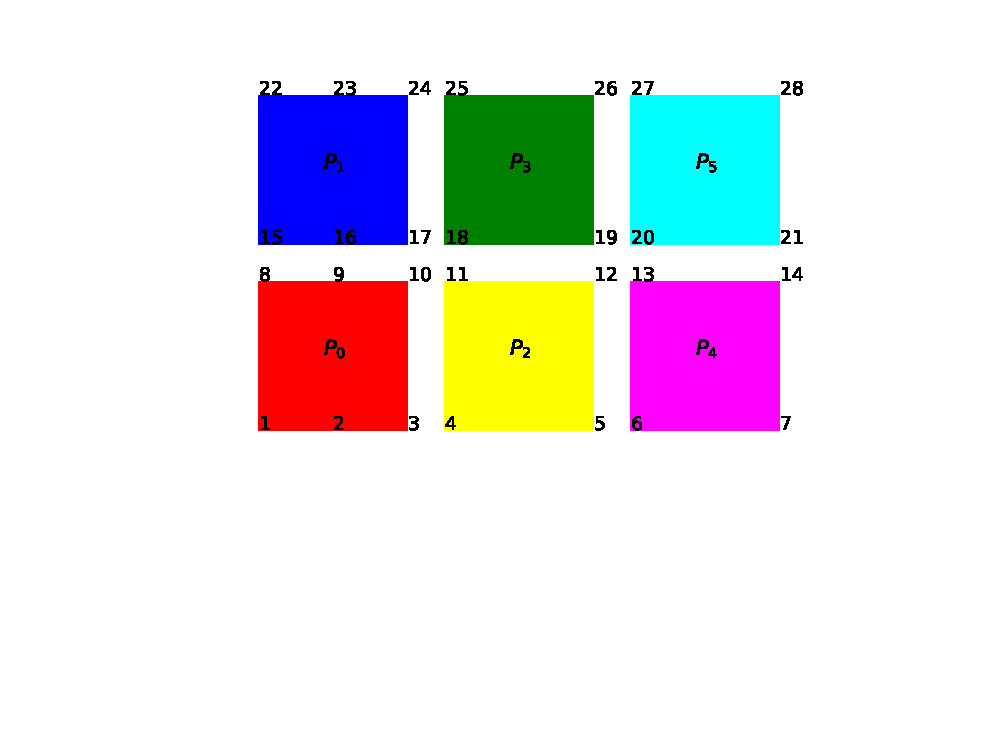
\includegraphics[angle=0,width=0.9\hsize]{figures/mpi_topology}
  \end{center}
  

\end{frame}
%******************************************************************

%******************************************************************
\begin{frame}
\frametitle{Vector Space Stencil}
\begin{itemize}
    \item Vector space for n-dimensional stencil format. Two different initializations
    are possible:
    \vskip 0.1cm
    - serial: \rule{0.4cm}{0pt} \textbf{\footnotesize StencilVectorSpace(npts, pads, dtype=float)}
        \vskip 0.1cm
    - parallel: \textbf{ \footnotesize StencilVectorSpace(cart, dtype=float)}
            \vskip 0.3cm

    \item Layer to which the local data structure belongs:
    \begin{itemize}
    \item [\ding{224}] Vector Stencil.
    \item [\ding{224}] Matrix Stencil.
    \end{itemize}

    \end{itemize}

\end{frame}
%******************************************************************

%******************************************************************
\begin{frame}
\frametitle{Vector Stencil}
  Partition of \emph{vectors} for the solution and RHS.
              \vskip 0.2cm

 \begin{itemize}
\item The $N_i+p_i$ Splines on each dimension are partitioned by
defining its starting and ending index $(s_i,e_i,\, i=1,2)$.

\item The size of the local 2D array holding the Splines
coefficients should be \emph{augmented} with \emph{ghost cells} of
widths $p_i$ at both ends of the vectors.
    \begin{itemize}
    \item [\ding{224}] Creation: \textbf{\footnotesize v = StencilVector(space)}.
    \item [\ding{224}] Local acess: $v[s_1:e_1, s_2:e_2]$
    \end{itemize}

\end{itemize}

\end{frame}
%******************************************************************


%******************************************************************
\begin{frame}
\frametitle{Matrix Stencil}
  Partition of the \emph{matrix} for linear operators.
  \vskip 0.2cm

  \begin{itemize}
  \item A quadratic bilinear operator.
    \begin{itemize}
    \item [\ding{224}] Creation: \textbf{\footnotesize M = StencilMatrix(space1, space2}).
    \item [\ding{224}] Local acess: $M[s_1:e_1, s_2:e_2, -p_1:p_1, -p_2:p_2]$
    \end{itemize}
    \item The \emph{local} matrix-vector product is thus defined simply by
\begin{align*}
    v_{i_1,i_2} = \sum_{k_1=-p_1}^{p_1}\!\sum_{k_2=-p_2}^{p_2}
    M_{i_1,i_2,k_1,k_2}\;u_{i_1+k_1,i_2+k_2}
  \end{align*}
where: $ s_1\le i_1\le e_1$ and $s_2\le i_2\le e_2$.
\end{itemize}
 
\end{frame}
%******************************************************************



%******************************************************************
\begin{frame}
\frametitle{Numurical illustrations}
 Solve a PDE equation:
\begin{eqnarray*}
\left\{
\begin{array}{r l}
-\triangle u + u  &= \quad  f \quad \text{in } \Omega
\\
\nabla u \cdot\textbf{n} & = \quad 0 \quad \text{on } \partial \Omega
\\
\end{array}
\right.
\end{eqnarray*}
\begin{itemize}
\item Computational domain: $\Omega = [0,1]^2$.
\item Discretization: Finite Element using B-Splines. 
\item Fine grid: $128x128$, coarse grid: $64x64$.
\item Smoother: PCG with Weighted Jacobi $(\omega = \frac{2}{3})$.
\item Post-smoother: PCG with GLT $(iterations = p+1)$.
\end{itemize}

\end{frame}
%******************************************************************

%******************************************************************
\begin{frame}
\frametitle{Scaling	Result}
\begin{itemize}
\item Assembly matrix $-\triangle + Id$ (Spline degree = 3, grid = 128x128):
\end{itemize}
  \begin{center}
    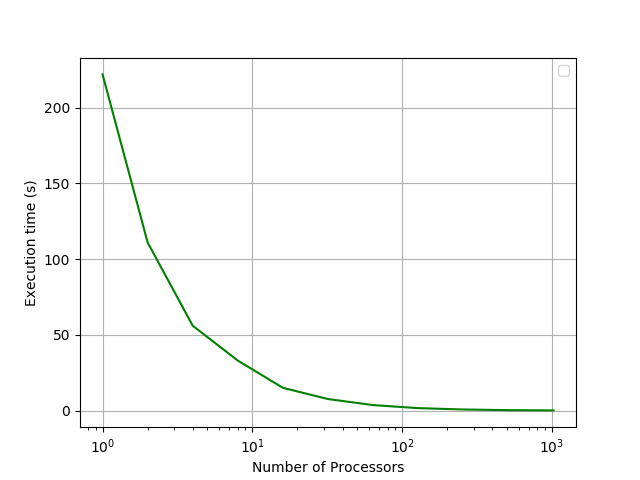
\includegraphics[angle=0,width=0.9\hsize]{figures/ass}
  \end{center}
\end{frame}
%******************************************************************

%******************************************************************
\begin{frame}
\frametitle{Scaling	Result}
\begin{itemize}
\item PCG + weighted Jacobi (iterations = $6$, tolernce = $10^{-6}$):
\end{itemize}
  \begin{center}
    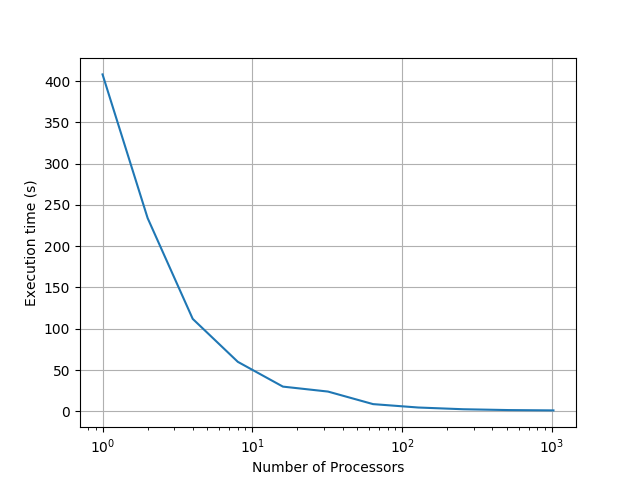
\includegraphics[angle=0,width=0.9\hsize]{figures/pres}
  \end{center}
\end{frame}
%******************************************************************

%******************************************************************
\begin{frame}
\frametitle{Scaling	Result}
\begin{itemize}
\item Smoother PCG + weighted Jacobi \textbf{vs.} Post-smoother PCG + GLT:
\end{itemize}
  \begin{center}
    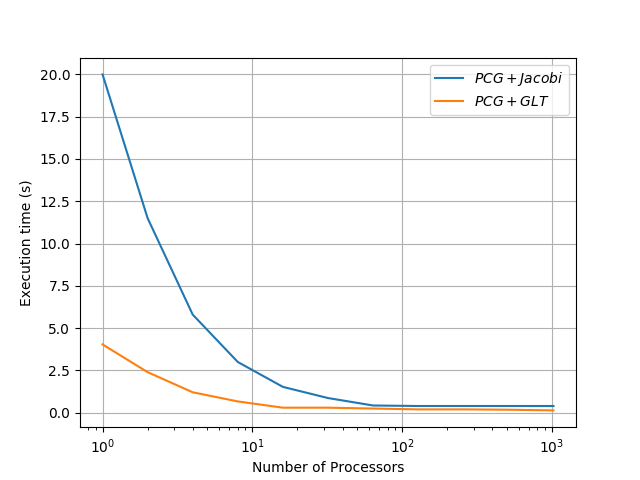
\includegraphics[angle=0,width=0.9\hsize]{figures/post1}
  \end{center}
\end{frame}
%******************************************************************

%******************************************************************
\begin{frame}
\frametitle{Scaling	Result}
\begin{itemize}
\item Post-smoother with different splines dregrees:
\end{itemize}
  \begin{center}
    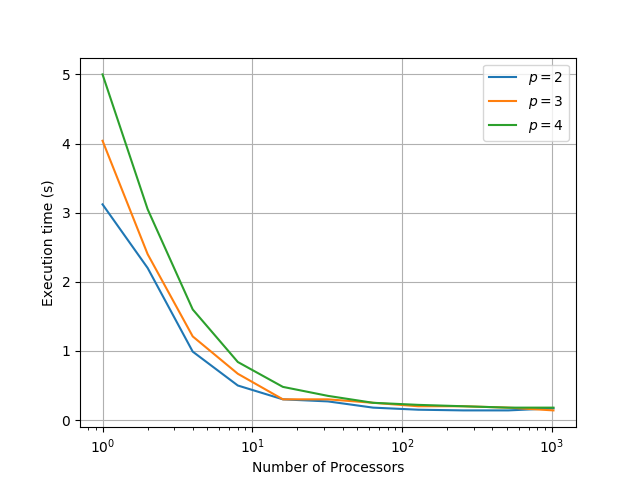
\includegraphics[angle=0,width=0.9\hsize]{figures/post2}
  \end{center}
\end{frame}
%******************************************************************

%******************************************************************
\begin{frame}
\frametitle{Conclusion and remarks}
\begin{itemize}
\item List of implemented and tested components:

\begin{itemize}
\item Inter-grid prolongation and restriction.
\item Parallel Jacobi relaxation.
\item Preconditioned PCG required for the GLT \emph{post-smoother}.
\item Prallelization patterns within isogeometric context
\begin{itemize}
\item[\ding{224}] Ghost cell exchange.
\item[\ding{224}] Local matrix-vector product.
\item[\ding{224}] Computation of residues.
\end{itemize}
\end{itemize}
\end{itemize}

\begin{itemize} 
\item Future works: 
\begin{itemize}
\item Perform more tests with various levels and discretizations.
\item Develop other parallel smoothers (Red-Black Jacobi, GMRES, ...).
\item Convert loops from Python to Fortran and accelerate the code using \emph{Pyccel} (tool like Pythran in {\small C++}).
\end{itemize}
\end{itemize}

\end{frame}

%******************************************************************

%******************************************************************
\begin{frame}
\frametitle{Benchmarks}
%
\footnotesize
\begin{table}[!ht] 
  \centering
  \begin{tabular}{c||c c c c c}
    \hline
            & Pure Python & Cython      & PyPy      & Pythran  & Pyccel
    \\\hline
     Timing &   0.12095        &  0.022737     &   0.017099      &  0.0012869    & \textbf{0.00096607} 
    \\
    Speedup &            &        &         &      &
    \\\hline
  \end{tabular}
  \caption{Benchmark result on the Black-Scholes program.}
%  \label{tab:<+label+>}
\end{table}
%

%
\begin{table}[!ht] 
  \centering
  \begin{tabular}{c||c c c c c}
    \hline
            & Pure Python & Cython      & PyPy      & Pythran  & Pyccel
    \\\hline
     Timing &    0.277       &  0.001811     &   0.059782     & 0.0024909   & \textbf{0.0007259} 
    \\
    Speedup &            &        &         &      &
    \\\hline
  \end{tabular}
  \caption{Benchmark result on the Grow-cut program.}
%  \label{tab:<+label+>}
\end{table}
%
%
\begin{table}[!ht] 
  \centering
  \begin{tabular}{c||c c c c c}
    \hline
            & Pure Python & Cython      & PyPy      & Pythran  & Pyccel
    \\\hline
    Timing  &   0.040508  &  0.0136299  &  0.147573 & 0.0294818 & \textbf{0.0048789} 
    \\
    Speedup &            &        &         &      &
    \\\hline
  \end{tabular}
  \caption{Benchmark result on the Rosen der program.}
%  \label{tab:<+label+>}
\end{table}
%
\end{frame}
%******************************************************************

%******************************************************************
%\begin{frame}

%{\huge
%Thank you!
%}
%\end{frame}
%******************************************************************




























\end{document}
